\documentclass[twoside]{article}
\usepackage{mathpazo}
\usepackage[T1]{fontenc}
\usepackage[utf8]{inputenc}
\usepackage{graphicx}
\usepackage[colorlinks]{hyperref}
\usepackage{caption} % unnumbered video examples
% \usepackage{authblk} % author affiliations
\usepackage{hanging} % hanging indents

% headers
\usepackage{fancyhdr}
\renewcommand{\headrulewidth}{0pt}

% first page footer
\fancypagestyle{infofooter}{%
  \fancyhf{}
  \renewcommand\headrulewidth{0pt}
  \fancyfoot[L]{\sffamily\small 
    WORLD MUSIC TEXTBOOK, ISSN: 2767-4215; \copyright~2021, CC-ND-BY-ND\\
    http://dx.doi.org/XX.XXXX/XXXXXXXX.2021.XXXXXXX}
}
\thispagestyle{infofooter} % remove header from first page
\pagestyle{fancy}     % add headers in other pages

% normal headers
\fancyhead[LO]{\sffamily\small \textbf{\thepage} \quad World Music Textbook}
\fancyhead[RE]{\sffamily\small Nielsen: Music and Identity in Danza Azteca \quad \textbf{\thepage}}
\fancyfoot{}

% flush left title
\makeatletter
\renewcommand{\maketitle}{\bgroup\setlength{\parindent}{0pt}
\begin{flushleft}
  \huge{\textbf{\@title}}

  \medskip
  
  \large{\@author}
\end{flushleft}\egroup
}
\makeatother

% for keywords
\providecommand{\keywords}[1]
{
  \newline
  \textbf{Keywords:} #1
}

% for link
\providecommand{\wmturl}[1]{
  \noindent\emph{The online version of this chapter includes all embedded content and is avaialble at #1.}
}

% metadata
\title{Music and Identity in Danza Azteca}
\author{Kristina F. Nielsen | Southern Methodist University}
% \affil{}

\date{}

% document
\begin{document}
\suppressfloats % prevent float above title
\maketitle

\paragraph{Abstract:}
  This piece considers how music contributes to identities within Aztec dance communities. It explores how different identities are created and sustained through music and dance practices.\keywords{dance, indigeneity, identity, tradition, Latin America, Native America, United States}

\medskip

\wmturl{https://worldmusictextbook.org/nielsen}

\noindent\hfil\rule{0.5\textwidth}{0.4pt}\hfil

\smallskip

In March 2016, I traveled from my home in Los Angeles, California, to
the annual Mexica New Year Celebration in San Jose, located about an
hour south of San Francisco. From the edge of the roped off circle, I
watched as my friends from Southern California danced to the
reverberating beats of the Aztec log drums, joining hundreds of other
dancers from across the United States. Together, they danced around the
drums in colorful regalia. While the New Year's celebration is a highly
social event with vendors and food, the dancing is also a form of
ceremony and offering, and danzantes sacrifice their bodily comfort
through hours of continuous dance. Each movement is accentuated through
the sounds of rattles on their legs, known as \emph{ayoyotes}, that are
made out of seedpods. As they dance, copal---a fragrant, ceremonial tree
sap---drifts through the air.

\begin{figure}
  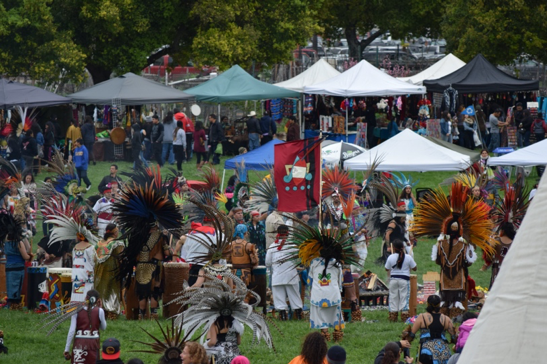
\includegraphics[width=\textwidth]{nielsen-fig1.jpg}
  \caption{Mexica New Year Ceremony in San Jose, California in March 2016}
\end{figure}

The \emph{Mexica} people ruled the Aztec Empire from the capital of
Tenochtitlan, and at its peak in the 1500s it spanned from the Pacific
Coast to the Caribbean. The Empire included Indigenous people of many
different cultures who paid tribute (similar to taxes) to the Mexica.
The Americas were forever changed with the arrival of Europeans in the
late 1400s. In 1519, Hernán Cortés arrived in Tenochtitlan with his
soldiers, often referred to as \emph{conquistadores}, and on August
13th, 1521, they defeated Tenochtitlan. Upon the ruins of the former
capital, the Spanish established present-day Mexico City as the new
capital of the colony of New Spain.

\begin{figure}
  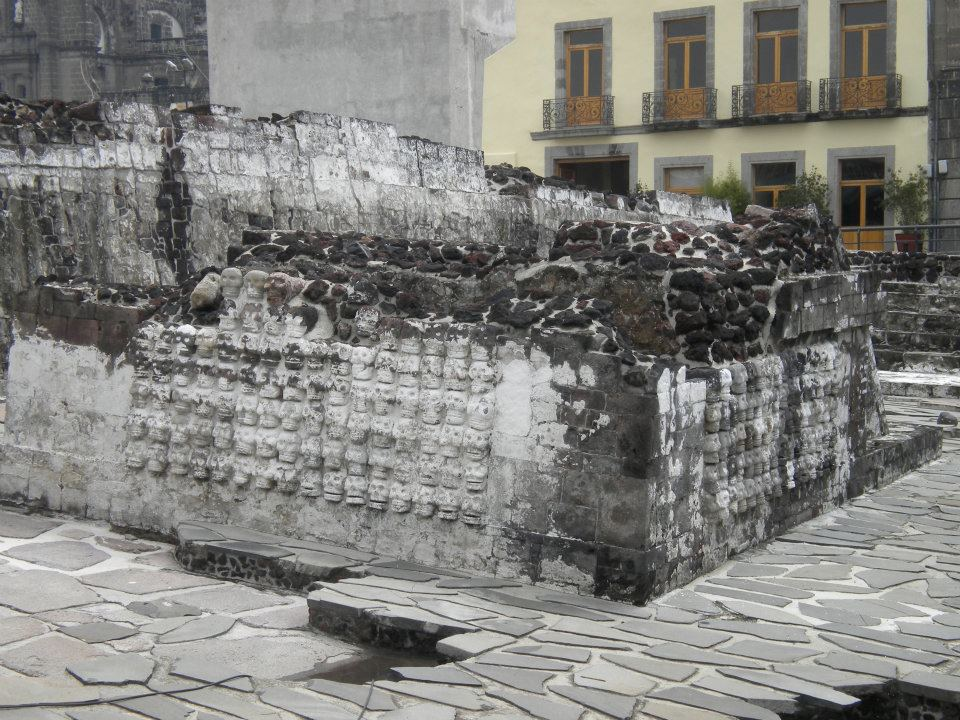
\includegraphics[width=\textwidth]{nielsen-fig2.jpg}
  \caption{The excavated ruins of a pyramid in the central square with a colonial-era building behind it}
\end{figure}

In the decades that followed the fall of Tenochtitlan, the Spanish
decimated traditional Mexica music and culture, which the Spanish
associated with the Devil (Sahagun trans. Anderson and Dibble 1951:207;
Tavárez 2011:35). Without the ability to time travel, it is virtually
impossible to know exactly what these dances may have been, what the
music sounded like, or what they meant to the Mexica. Nonetheless, there
are many song texts, artifacts, documentation of Mexica spirituality,
descriptions of music and dance performances, and images of musicians
and dancers.\footnote{This does not mean that there is not continuity,
  only that without reliable sources these continuities cannot be
  verified. For analyses that have explored how continuity might be
  determined, see Grazia Tuzi's \emph{The Voladores Dance: Traces of the
  Past for the Interpretation of the Present} (2013) and a deeper
  exploration of the idea of continuity and breaks in the danza
  tradition (Nielsen 2014).}

These images and descriptions of music and dance gained significance in
the twentieth century after the Mexican Revolution. Following decades of
conflict, the political leadership of Mexico sought to unite the many
diverse communities across Mexico through a single shared national
identity (Gamio {[}1916{]}2010; Klor de Alva 1992; Alonso 2004). To
achieve this goal, Mexico and its nationalist thinkers forwarded the
concept of \emph{mestizaje}, or European and Indigenous racial and
cultural mixing (Vasconcelos {[}1925{]}1979; Brading 1988).\footnote{There
  are large African and Asian communities in Mexico who have made
  important cultural contributions to music and dance. While these are
  sometimes included in the idea of \emph{mestizaje}, they were
  discriminated against by many Mexican national thinkers in the early
  twentieth century and not fully included in the national ideology of
  mestizaje (Vasconcelos 1979:43-44; Knight 1990:97). For that reason, I
  focus on Europeans and Spanish traditions that are important to Danza
  Azteca.} In pursuit of this goal, musicians, artists, and dancers in
Mexico City turned to symbols from the Aztec Empire to shape a shared
national cultural heritage (See González Torres 2005; Rostas 2009;
Saavedra 2015).

Despite the push for cultural homogeneity from national leadership,
Mexico remains a pluricultural society. Today there are more than
seventeen million Indigenous people in Mexico who speak over sixty-eight
Indigenous languages (Working Group on Indigenous Populations 1995;
Instituto Nacional de Lenguas Indígenas Nacionales 2008). For official
recognition as Indigenous peoples, communities and individuals must meet
a number of criteria required by nations and international
organizations. For instance, to receive official recognition, the United
Nations requires self-identification as Indigenous as well as acceptance
of the claim by the community (United Nations Permanent Forum on
Indigenous Issues). They also require historical continuity extending to
before colonialism, connections to land and territories, and cultural
continuity including language, rituals, and social structures (ibid.).
On a national level, Mexico continues to confer Indigenous status
predominantly based upon the ability to speak an Indigenous language
(Comisión Nacional para el Desarrollo de los Pueblos Indígenas
2006:131). In contrast, the United States federal government recognizes
Indigenous people---also known as Native Americans or American
Indians---predominantly through heritage, including metrics like ``blood
quantum'' (Garoutte 2003:15). While virtually all of the danzantes have
Indigenous Mexican ancestry, very few participants in Danza Azteca meet
the stringent requirements of the United Nations or national governments
for official recognition as Indigenous individuals.

Bearing these contexts in mind, what are danzantes performing at
gatherings like the Mexica New Year Ceremony given that Mexica music and
ritual culture was decimated following the arrival of the Spanish? And
what do these performances reveal regarding the significance of music
and dance in shaping how danzantes think about their identities and
Indigenous heritages? In this essay, I unpack these two critical
questions using a theoretical framework known as ``articulation
theory.'' This theoretical framework was developed by Stuart Hall, a
British-Jamaican sociologist and cultural studies researcher who worked
extensively with understandings of identity, popular culture, and race
(Hall 1986; Grossberg 1996; DeLuca 1999; Clarke 2015). Drawing on Hall's
work, I explore the ways in which music and dance have come to play
critical roles in shaping identities within Danza Azteca communities.

\hypertarget{music-at-the-mexica-new-year-ceremony}{%
\section*{Music at the Mexica New Year
Ceremony}\label{music-at-the-mexica-new-year-ceremony}}

\begin{figure}
  
\includegraphics[width=\textwidth]{play-video.png}
  \caption*{Video Example 1. Example of a dance from the 2016 Mexica New Year
  Ceremony in San Jose, California hosted by Calpulli Tonalehqueh}
\end{figure}

As can be heard in Video Example 1, the music at the Mexica New Year
ceremony meets many expectations listeners might have for what an
ancient Aztec music should sound like. The instruments the musicians
play are replicas, or models, of historical instruments from across
Mesoamerica that are commonly found in museum collections today.
Additionally, instruments that have European origins, such as string
instruments, are largely absent, even though they were important in a
key predecessor to Danza Azteca, known as conchero. Furthermore, many
songs at the ceremony are sung in Nahuatl, the language spoken by the
Mexica (González Torres 2005; Rostas 1991, 2009).

Since the arrival of Europeans, Indigenous music has become intertwined
with European music through a process known as \emph{syncretism}. In
short, syncretism combines two or more cultures into a new cultural
entity. In Central Mexico, Indigenous musicians adapted string
instruments into their music, and Indigenous spiritual beliefs blended
with Catholicism. For instance, Conchero communities blended Indigenous
spiritual beings with Jesus and Catholic saints (Stone 1975:195). The
Aztec musicians I have spoken with in Los Angeles have experimented with
instruments and what music may have sounded like prior to European
musical and religious influences. Many musicians who perform on Aztec
instruments have conducted extensive research on Aztec history and
spirituality, the Nahuatl language, and music. In their research, they
draw heavily on historical sources, including accounts from the colonial
era that were written by both Indigenous and Spanish observers. They
also draw on music and dances from the many Indigenous communities in
Mexico---and even sometimes the United States---that continue to the
present day. These efforts are particularly complicated since cultures
and traditions are always changing, even if only ever so slightly. While
many Indigenous cultures in Central Mexico continue traditions that
likely originated before the arrival of the Spanish, these traditions
are unlikely to have been exactly the same as Mexica rituals or musical
practices in Tenochtitlan.

\begin{figure}
  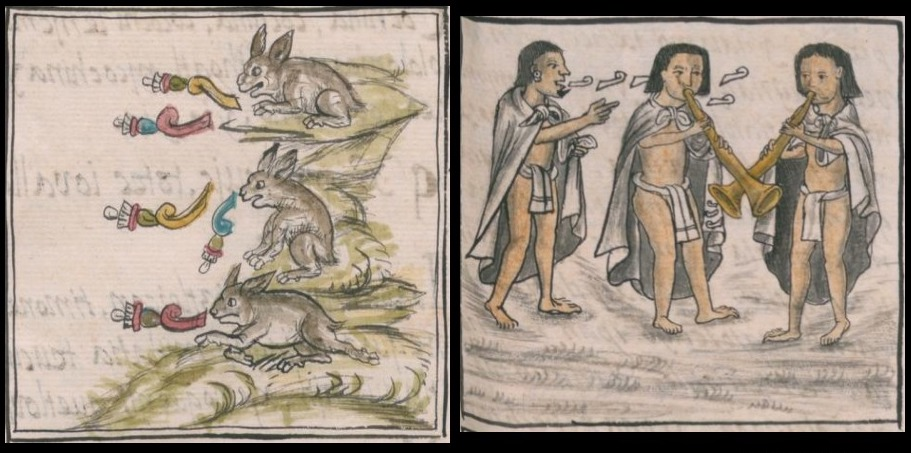
\includegraphics[width=\textwidth]{nielsen-fig3.jpg}
  \caption{Images from the Florentine Codex that was written in the 1500s by Nahua scribes}
\end{figure}

In addition to written and community sources, musicians performing on
Mesoamerican instrument replicas also draw on their own creativity,
experiences, identities, and interpretation of what the Aztec past might
have been like. For instance, Carlos Daniel Jimenez Vasquez, a danzante
who also plays an array of Indigenous instruments, shared that he tries
to imagine what a dance might reflect and integrates instruments
accordingly. He considers events like battles or celebrations and tries
to describe them musically (Personal Interview 2015). Vasquez also
performs music that draws on his Zapotec heritage from his hometown of
Maquilxochitl in the state of Oaxaca. In particular, he draws
inspiration from traditional flute music from Oaxaca. While Vasquez is
fully of Zapotec descent, he did not learn the language and he is not
eligible for official recognition as Indigenous in the United States.

Cuezalin, another danzante and musician, similarly draws on his
Indigenous Cora-Tepehuan heritage. Cuezalin has conducted extensive
research with historical texts to inform his composition of new dances
and songs. Cuezalin lives in Santa Ana where he leads a dance community
called Xiuhcoatl, meaning ``turquoise serpent'' in Nahuatl. At the
Mexica New Year ceremony, Cuezalin led a dance and song called ``Zan
Yehuan'' that he developed along with companions in a group called the
Xochimecayahualli from Southern California (Personal Interview 2015)
(see Video Example 2). The song draws on a Nahuatl text by the king and
poet Nezahualcoyotl who governed the city of Texcoco in the 1500s
(León-Portilla 1992:97). To adapt the song text for modern performance,
Cuezalin and the Xochimecayahualli have shifted lines of the text,
composed a new melody, and added dance steps. In the performance, the
dancers move in an interlocked line holding hands. Cuezalin then
transitions this dance to a popular Mexican song ``La Víbora'' or ``the
snake'' that uses the same rhythms and dance steps.

\begin{figure}
  
\includegraphics[width=\textwidth]{play-video.png}
  \caption*{Video Example 2. Cuezalin leading ``Zan Yehuan'' at the Mexica New
  Year Ceremony in San Jose, California}
\end{figure}

\hypertarget{danza-and-articulation-theory}{%
\section*{Danza and Articulation
Theory}\label{danza-and-articulation-theory}}

Stuart Hall's articulation theory provides one useful vantage point for
considering the ways in which music and dance are shaping how danzantes
interpret their identities. Hall suggested that identities and
communities are constantly being formed by coupling and decoupling
different elements together (Hall 1986; Grossberg 1996). Hall likened
this process to a truck with multiple interchangeable trailers in a
conversation with fellow sociologist Lawrence Grossberg (1996). Hall
points out that these elements are not permanently fused but rather
flexible. New elements can be coupled together (and in turn decoupled),
and in the process they can change how individuals and communities
identify.

Articulation theory provides a way of thinking about these music and
dance elements that are being connected by individuals and communities
within Danza Azteca. Danzantes can identify with Mexican national
heritage through the Aztec symbols promoted in twentieth-century
nation-building projects. They can also identify with their Indigenous
heritages through these same performances. This can provide a forum for
celebrating Indigenous ancestors despite not meeting the strict criteria
for Indigenous recognition. Music and dance become important resources
for navigating the challenges many danzantes face in having Indigenous
heritage and culture yet not receiving recognition. Through music and
dance, danzantes celebrate their heritage while circumventing and
challenging Mexican and U.S. definitions of Indigenous people that
frequently overlook Indigenous cultures in Mexico and along the U.S.
Mexican border.

``Zan Yehuan'' from the Mexica New Year ceremony is an example where
music and dance offer insight into how diverse elements of the
danzantes' individual and communal identities are combined. All the
elements---the ancient Nahuatl text, the new melody composed in Southern
California by Cuezalin and the Xochimecayahualli, and the heartbeat
rhythm---connect danzantes with different aspects of their Indigenous
heritages through the umbrella of Aztec culture. Cuezalin and other
musicians draw from their own Indigenous heritages and their personal
creativity. Cuezalin and the Xochimecayahualli simultaneously draw on
the Nahuatl text to forge a relationship with the past. I interviewed
Cuezalin about these songs, and he shared why this text is so meaningful
to him:

\begin{quote}
I believe that their power is in the connection they establish to the
words of the ancients. And when we pronounce the words that they
pronounced, that for them were special, when we sing their songs we are
transported to an ancient time---to a time that unites many of us that
are descended from the Aztecs, so to speak, the people that spoke in
those times. Even though our ancestors may not have been Nahuatl
speakers at that time, these are words that were spoken in the time that
our ancestors lived. Therefore, they transport us like a time capsule
\ldots{} It is a gem, a physical thing that can be sung, that one can
say. Someone might, for example, have a mask or a piece of old jade, but
only one person can have that. A song is different. A song can belong to
many people, and you can protect it and care for it. That is the power
of the spoken word. (Personal Interview with Cuezalin 2015)
\end{quote}

\begin{figure}
  
\includegraphics[width=\textwidth]{play-video.png}
  \caption*{Video Example 3. Cuezalin performing ``Zan Yehuan'' and discussing the origins of the song}
\end{figure}

At the same time, as demonstrated and discussed by Cuezalin in Video
Example 3, the transition into ``La Víbora'' highlights a shared Mexican
identity, using a song common in Mexican celebrations, such as weddings.
For danzantes, these musical elements and their interwoven identities,
both ethnic and national, are not exclusive: They exist simultaneously.
Through music and dance, danzantes can emphasize one element and then
another, using music to temporarily bring different aspects of their
identities to the forefront while simultaneously celebrating all of them
collectively.

\hypertarget{additional-materials}{%
\section*{Additional Materials}\label{additional-materials}}

\hypertarget{discussion-questions}{%
\subsection*{Discussion Questions}\label{discussion-questions}}

\begin{enumerate}
\def\labelenumi{\arabic{enumi}.}
\item
  Consider the many different types of music that you listen to and
  perform in the different settings of your life \emph{(religious
  services, family functions, cultural or ethnic celebrations, hanging
  out with college friends v. childhood friends, and other communities
  in which you participate)}.

  \begin{itemize}
  \item
    In what ways does your identity change in these different settings?
  \item
    What are some ways in which you may be coupling and decoupling
    elements together to shape your identity through music?
  \end{itemize}
\item
  As we explored above, history is a frequent theme in Danza Azteca. Why
  do you think history is so important to the danzantes?

  \begin{itemize}
  \item
    Can you think of other examples, possibly from your own life, where
    a song or piece of music is important to you or others because of
    its history?
  \end{itemize}
\end{enumerate}

\hypertarget{recommended-readings}{%
\subsection*{Recommended Readings}\label{recommended-readings}}

\hangpara{15pt}{1} Garroutte, Eva Marie. 2003. \emph{Real Indians: Identity and
the Survival of Native America}. Berkeley: University of California
Press.

\hangpara{15pt}{1} Nájera-Ramírez, Olga, Norma Elia Cantú and Brenda M. Romero,
eds.~2009. \emph{Dancing Across Borders: Danzas y Bailes Mexicanos}.
Urbana: University of Illinois Press.

\hangpara{15pt}{1} Scolieri, Paul A. 2013. \emph{Dancing in the New World:
Aztecs, Spaniards, and the Choreography of Conquest.} Austin: University
of Texas Press.

\hypertarget{digital-resources}{%
\subsection*{Digital Resources}\label{digital-resources}}

\hangpara{15pt}{1} \emph{\href{https://www.wdl.org/en/item/10096/}{General
History of the Things of New Spain by Fray Bernardino de Sahagún: The
Florentine Codex}}. World Digital Library.

\begin{quote}
A digitized version of the Florentine Codex, which was drafted in the
1500s by Indigenous scribes and the monk Bernardino de Sahagún in the
decades following the fall of Tenochtitlan. This book describes the
religion, life, history, and songs of Nahua people of Central Mexico.
\end{quote}


\hangpara{15pt}{1} \href{https://archive.org/details/calauem_201702_item_16_6-9/DSC_0003_Cuezalin+talking+about+and+playing+Maquil+Xochitl+and+Nayeli.MOV}{\emph{UCLA
Ethnomusicology Archive, Collection 2017.02}}. Collected by Kristina
Nielsen.

\begin{quote}
Watch Cuezalin discuss his composition process and demonstrate rhythms
and dances.
\end{quote}

\hypertarget{works-cited}{%
\section*{Works Cited}\label{works-cited}}

\begin{hangparas}{15pt}{1}
 Alonso, Ana María. 2004. ``Conforming Disconformity:
`Mestizaje,' Hybridity, and the Aesthetics of Mexican Nationalism.''
\emph{Cultural Anthropology} 19(4): 459-90.

 Brading, David A. 1988. ``Manuel Gamio and Official
Indigenismo in Mexico.'' \emph{Bulletin of Latin American Research}
7(1): 75-89.

 Clarke, John. 2015. ``Stuart Hall and the Theory and Practice
of Articulation.'' \emph{Discourse: Studies in the Cultural Politics of
Education} 36(2): 275-286.

 Comisión Nacional para el Desarrollo de los Pueblos
Indígenas. 2006.
\href{http://www.cdi.gob.mx/idh/informe_desarrollo_humano_pueblos_indigenas_mexico_2006.pdf}{``Informe
sobre desarrollo Humana de los pueblos indígenas de México.''} Accessed
6 May 2020.

 DeLuca, Kevin. 1999. ``Articulation Theory: A Discursive
Grounding for Rhetorical Practice.'' \emph{Philosophy \& Rhetoric}
32(4): 334-48.

 Gamio, Manuel. 2010. \emph{Forjando Patria:
Pro-Nacionalismo}, translated by Fernando Armstrong-Fumero. Boulder:
University Press of Colorado.

 González Torres, Yólotl. 2005. \emph{Danza Tu Palabra: La
Danza de Los Concheros}. Mexico City: Conaculta-INAH.

 Grossberg, Lawrence. 1996. ``On Postmodernism and
Articulation: An Interview with Stuart Hall.'' In \emph{Stuart Hall:
Critical Dialogues in Cultural Studies}, edited by David Morley and
Kuan-Hsing Chen, 131-51. New York: Routledge.

 Hall, Stuart. 1986. ``Gramsci's Relevance for the Study of
Race and Ethnicity.'' \emph{Journal of Communication Inquiry} 10(2):
5-27.

 Hall, Stuart. 2002. ``Race, Articulation and Societies
Structured in Dominance.'' In \emph{Race Critical Theories: Text and}
Context, edited by Philomena Essed and David Theo Goldberg, 38-68.
Oxford: Blackwell Publishers.

 International Work Group for Indigenous Affairs. 2019.
\href{https://www.iwgia.org/en/mexico.html}{``Indigenous Peoples in
Mexico.''} Accessed April 9, 2020.

 Instituto Nacional de Lenguas Indígenas Nacionales. 2008.
\href{https://www.inali.gob.mx/pdf/CLIN_completo.pdf}{``Catálogo de las
Lenguas Indígenas Nacionales: Variantes Lingüísticas de México con sus
Autodenominaciones y Referencias Geoestadísticas.''} \emph{Diario
Oficial}. Accessed April 9, 2020

 Klor de Alva, J. Jorge. 1992. ``Introduction: Nahua Studies,
The Allure of the `Aztecs,' and Miguel León-Portilla.'' In \emph{The
Aztec Image of Self and Society: An Introduction to Nahua Culture},
edited by J. Jorge Klor de Alva, vii-xxiii. Salt Lake City: University
of Utah Press.

 Knight, Alan. 1990. ``Racism, Revolution, and Indigenismo:
Mexico, 1910-1940.'' In \emph{The Idea of Race in Latin America,
1870-1940}, edited by Richard Graham, 71-113. Austin: University of
Texas Press.

 León-Portilla, Miguel. 1992. \emph{Fifteen Poets of the Aztec
World}. Norman: University of Oklahoma Press.

 Nielsen, Kristina. 2014.
\href{https://ethnomusicologyreview.ucla.edu/content/role-interpretation-determining-continuity-danza-azteca-history}{``The
Role of Interpretation in Determining Continuity in Danza Azteca
History.''} \emph{Ethnomusicology Review}. Accessed April 9, 2020

 Rostas, Susana. 1991. ``The Concheros of Mexico: A Search for
Ethnic Identity.'' \emph{Dance Research: The Journal of the Society for
Dance Research} 9(2): 3-17.

 ­­­------. 2009. \emph{Carrying the Word}. Boulder:
University of Colorado Press.

 ­­­------. 2002. ``\,`Mexicanidad' The Resurgence of the
Indian in Popular Mexican Nationalism.'' \emph{The Cambridge Journal of
Anthropology} 23(1): 20-38.

 Saavedra, Leonora. 2015. ``Carlos Chávez and the Myth of the
Aztec Renaissance.'' In \emph{Carlos Chávez and His World}, edited by
Leonora Saavedra, 134-165. Princeton: Princeton University Press.

 Sahagún, Bernardino de. 1951 {[}1540-1585{]}.
\emph{Florentine Codex Book II} translated by Arthur Anderson and
Charles Dibble. Santa Fe: The School of American Research and the
University of Utah.

 Tavárez, David. 2011. \emph{The Invisible War: Indigenous
Devotions, Discipline, and Dissent in Colonial Mexico}. Stanford:
Stanfor University Press.

 Tuzi, Grazia. 2013. ``The \emph{Voladores} Dance: On the Use
of Evidence from the Past to Interpret the Present.'' In \emph{Flower
World: Music Archaeology of the Americas} Volume 2, edited by Matthias
Stöckli and Arnd Adje Both, 159-176. Berlin: Ekho Verlag.

 United Nations Permanent Forum on Indigenous People.
\href{https://www.un.org/esa/socdev/unpfii/documents/5session_factsheet1.pdf}{``Factsheet.''}
Accessed April 9, 2020.

 Vasconcelos, José. 1979 {[}1925{]}. \emph{The Cosmic Race: La
raza cósmica}. Trans. Didier T. Jaén. Baltimore: John Hopkins University
Press.
\end{hangparas}

\end{document}